\documentclass{article}
\usepackage{amsmath}
\usepackage{tikz}
\usetikzlibrary{calc}

\begin{document}

\begin{center}
    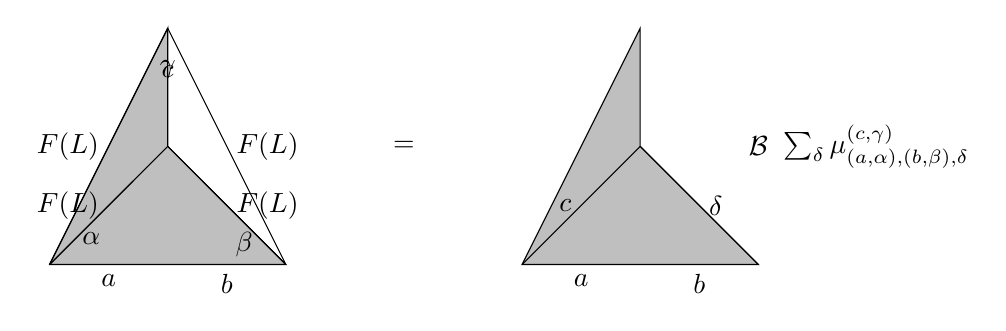
\begin{tikzpicture}[scale=1.5]
        % Define coordinates
        \coordinate (A) at (0,0);
        \coordinate (B) at (2,0);
        \coordinate (C) at (1,1);
        \coordinate (D) at (1,2);
        
        % Draw the parallelogram
        \draw[fill=gray!50] (A) -- (B) -- (C) -- (D) -- cycle;
        
        % Draw the lines and labels
        \draw (A) -- (C) node[midway, left] {$F(L)$};
        \draw (B) -- (C) node[midway, right] {$F(L)$};
        \draw (A) -- (D) node[midway, left] {$F(L)$};
        \draw (B) -- (D) node[midway, right] {$F(L)$};
        
        \draw (C) -- (D) node[midway, above] {$c$};
        \draw (C) -- ($(C)!1cm!(D)$) node[midway, above] {$\gamma$};
        
        \draw (A) -- ($(A)!1cm!(B)$) node[midway, below] {$a$};
        \draw (B) -- ($(B)!1cm!(A)$) node[midway, below] {$b$};
        
        \draw (A) -- ($(A)!1cm!(C)$) node[midway, below] {$\alpha$};
        \draw (B) -- ($(B)!1cm!(C)$) node[midway, below] {$\beta$};
        
        \node at (3,1) {$=$};
        
        \begin{scope}[xshift=4cm]
            % Define coordinates
            \coordinate (E) at (0,0);
            \coordinate (F) at (2,0);
            \coordinate (G) at (1,1);
            \coordinate (H) at (1,2);
            
            % Draw the parallelogram
            \draw[fill=gray!50] (E) -- (F) -- (G) -- (H) -- cycle;
            
            % Draw the lines and labels
            \draw (E) -- (G) node[midway, left] {$c$};
            \draw (F) -- (G) node[midway, right] {$\delta$};
            
            \draw (E) -- ($(E)!1cm!(F)$) node[midway, below] {$a$};
            \draw (F) -- ($(F)!1cm!(E)$) node[midway, below] {$b$};
            
            \node at (3,1) {$\sum_{\delta} \mu_{(a,\alpha),(b,\beta),\delta}^{(c,\gamma)}$};
        \end{scope}
        
        \node at (6,1) {$\mathcal{B}$};
    \end{tikzpicture}
\end{center}

A multiplication on \( F(L) \) is determined by the complex numbers \( \mu_{(a,\alpha),(b,\beta),\delta}^{(c,\gamma)} \).

\end{document}